\documentclass[tikz,border=2pt]{standalone}
\usepackage{amsmath,amssymb}
\usepackage{tikz}

\begin{document}
% Discrete metric: every two distinct points are at distance exactly 1, so a ball of radius
% 1/2 contains only its centre and every set is open.
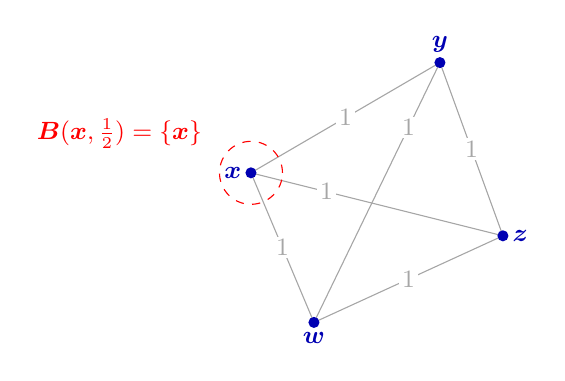
\begin{tikzpicture}[every node/.style={font=\small}]
	\coordinate (a) at (0,0); \coordinate (b) at (2.4,1.4); \coordinate (c) at (3.2,-0.8); \coordinate (d) at (0.8,-1.9);
	\foreach \p/\q/\t in {a/b/0.5, a/c/0.3, a/d/0.5, b/c/0.5, b/d/0.25, c/d/0.5} {\draw[gray!70] (\p) -- (\q) node[pos=\t, fill=white, inner sep=1pt] {$1$};}
	\foreach \p/\l in {a/$\boldsymbol{x}$, b/$\boldsymbol{y}$, c/$\boldsymbol{z}$, d/$\boldsymbol{w}$} {\fill[blue!70!black] (\p) circle (2pt);}
	\node[blue!70!black, left] at (a) {$\boldsymbol{x}$};
	\node[blue!70!black, above] at (b) {$\boldsymbol{y}$};
	\node[blue!70!black, right] at (c) {$\boldsymbol{z}$};
	\node[blue!70!black, below] at (d) {$\boldsymbol{w}$};
	\draw[red, dashed] (a) circle (0.4);
	\node[red, anchor=east] at (-0.5,0.5) {$\boldsymbol{B}(\boldsymbol{x},\tfrac12)=\{\boldsymbol{x}\}$};
\end{tikzpicture}
\end{document}
